\chapter{前提知識}
以下では,
本書で想定しているコンピュータのハードウェアやソフトウェアの
構成について解説する.

\section{コンピュータのハードウェア構成}
本書は,
コンピュータのハードウェア構成が\figref{hardBlock}のようになっている
ことを前提にしている.
複数のCPU(Central Processing Unit)がメモリを共有し,
また,全てのCPUは同じ機能を持ち優劣が無い.
このような方式を
{\bf SMP(対称型マルチプロセッシング:Symmetric Multiprocessing)}と呼ぶ.
メモリはCPUだけでなく,
I/Oコントローラ(\figref{hardBlock}ではアダプタやコントローラ)にも
共有される.

\myfigure{btp}{scale=0.48}{Fig/hardBlock-crop.pdf}{ハードウエア構成}{hardBlock}

\begin{enumerate}
\item CPU \\
CPUはコンピュータの頭脳である.
図はCPUが二つの構成になっているが,
実際は一つの場合も,もっと多い場合もある.

\item メモリ(主記憶装置) \\
プログラムやデータを記憶し,
プログラム実行する際にCPUが直接使用する記憶装置である.

\item タイマー \\
一定間隔で繰り返しCPUに割り込みを発生するインターバルタイマーである.

\item グラフィックアダプタ \\
ディスプレイを接続するためのアダプタである.
表示内容を記憶するメモリを独自に持つ場合と,
主記憶装置を使用する場合がある.
最近のパーソナルコンピュータでは,
グラフィックアダプタにGPU(Graphics Processing Unit)が組込まれている.

\item SATA ホストコントローラ \\
SATA(Serial Advanced Technology Attachment)は,
パーソナルコンピュータと二次記憶装置(ハードディスクやCD-ROM)を接続するための
インタフェース規格である.
SATA ホストコントローラは次のような動作をする.
\begin{enumerate}
\item CPUがSATAホストコントローラにコマンドを書き込む.
コマンドは,
「読み/書き」,「セクタアドレス」,「セクタ数」,「メモリアドレス」
を含んだものである.
\item SATAホストコントローラは,
ディスクコントローラと通信しハードディスクにコマンドを渡す.
\item ハードディスクの読み・書きが可能になったら,
ホストコントローラはハードディスクとメモリの間でデータ転送を行う.
このようなCPUを介さないデータ転送のことを,
{\bf DMA(Direct Memory Access)}\label{dma}と呼ぶ.
\item SATAホストコントローラはCPUに割り込み信号を送り,
データの転送が完了したことを知らせる.({\bf I/O完了割り込み})
\end{enumerate}
CPUは,
SATAホストコントローラにコマンドを送ってから割り込みが発生するまでの間,
他の仕事をすることができる.
ハードディスクの操作(I/O操作)とCPUの計算は並列実行される.

\item USBコントローラ \\
USB(Universal Serial Bus)は,
パーソナルコンピュータと周辺装置を手軽に接続できるインタフェースである.
USBメモリスティックやプリンタ,キーボード,マウス等,多くの周辺装置が
USBを通して接続できる.
USBコントローラもSATAホストコントローラのようにDMA機能を備えている.

\item ネットワークアダプタ \\
パーソナルコンピュータのネットワークアダプタは,
GbE(Gigabit Ethernet)規格のものが普及している.
これもSATAホストコントローラのようにDMA機能を備えている.

\item BUS(バス) \\
パーソナルコンピュータのハードウェアを構成する装置の間で
データをやり取りするための配線である.
CPUだけでなくDMAを使用するコントローラやアダプタが大量のデータ転送を行うので,
バスのデータ転送能力がパーソナルコンピュータの性能向上のボトルネックになる.

そのため後で説明するように,実際の物理的な接続は\figref{hardBlock}とは
かなり異なった構成になっている.
しかし,オペレーティングシステムが意識しなければならない論理的な
接続は\figref{hardBlock}のようなものである.

\end{enumerate}

\section{CPUの構成}
本書では、CPUは\figref{cpuBlock}のような部品で構成されると考える.
\figref{hardBlock}に示したように,CPUはBUSを通して他の装置と接続される.
CPUは,一つの機械語命令の実行が終わり次の命令の実行を開始する前に,
他の装置から割り込みを受け付けることができる\footnote{
例外的に,メモリ管理に関する一部の割込は機械語命令の途中で発生する.}.

\myfigure{btp}{scale=0.66}{Fig/cpuBlock-crop.pdf}{CPUの構成}{cpuBlock}

\begin{enumerate}
\item {\bf PSW(Program Status Word)} \\
PSWは,PC(Program Counter)とFlags(フラグ)から構成されるものとする
\footnote{
教科書によっては,フラグだけをPSWと呼ぶ場合もある.}.
PCはCPUが実行中のプログラムの命令アドレスを保持するカウンタである.
Flagsは計算の結果によって変化するフラグの他に,
割り込み許可/不許可を表現するビット,
実行モード(ユーザモード/カーネルモード)を表現するビット等が含まれる.

\item {\bf CPUレジスタ} \\
計算に使用するCPUの汎用レジスタのことである.
TeCではG0,G1,G2,SPのこと,
情報処理技術者試験のCOMETではGR0,GR1,GR2,GR3,GR4のことである.

\end{enumerate}

PSWとCPUレジスタは,
機械語命令を実行する毎に値が変化・確定しプログラムが意識している\footnote{
一方でCPU内部にはプログラムから見えないレジスタもある.
}ので,CPUを仮想化し実行するプロセスを切換える際に保存・復旧の対象となる.

\section{最近のコンピュータの実際の構成}

Intel社のCPUを使用したデスクトップ・パーソナルコンピュータと
サーバコンピュータの構成を説明する.
バスがボトルネックにならないように,
CPUにメモリを直接接続してある.

\subsection{デスクトップ・パーソナルコンピュータ}
\figref{intelDesktop}はIntel社のCPUを使用した
近年のデスクトップ・パーソナルコンピュータの構成を表している.
Intel社の用語では,これまで「CPU」と呼んでいたものを
「{\bf Core(コア)}」と呼ぶ.
「CPU」は複数のコアを含んだLSIのことを指している.
デスクトップ用のCPUには1〜4個のコアが集積されている.

コアに隣接しているL1はレベル1キャッシュ(Level 1 cache)を表している.
L2は複数のコアにシェアされるレベル2キャッシュ(Level 2 cache)を表している.
メモリとのデータ転送量が多いCoreとGPUがCPUに集積され,
I/O装置のコントローラやアダプタはPCHに集積されている.
CPUとPCHはDMIと呼ばれる専用のインタフェースを用いて接続される.

\myfigure{btp}{scale=0.66}{Fig/intelDesktop-crop.pdf}
{デスクトップPCの構成}{intelDesktop}

\subsection{サーバコンピュータ}
より強力な処理能力が必要なサーバ用コンピュータでは,
\figref{intelServer}のように多くのコアを内蔵するCPUを複数個使用する.
現在(2017年秋)最新の Intel Xeon Processor Scalable Family の場合,
CPU同士はUPIと呼ばれる高速な専用インタフェースで接続される.
最大の構成は,28コアのCPUを8個使用し合計224コアのものである.
PCHもサーバ用のものでは,より多くのストレージやネットワークを接続できる.

\myfigure{btp}{scale=0.5}{Fig/intelServer-crop.pdf}
{サーバPCの構成}{intelServer}

\section{オペレーティングシステムの構造}
\figref{osOrganization}にオペレーティングシステムの構造を示す.
オペレーティングシステムのカーネルは
\figref{osOrganization}中央部分のソフトウェアである.
ユーザプロセスはユーザモードで,
カーネルはカーネルモードで実行される.

\subsection{カーネルの構成}
\figref{osOrganization}に示すように,
カーネルは以下のようなモジュールから構成される.

\begin{enumerate}
\item {\bf 割り込みハンドラ} \\
割込みが発生した時に自動的に実行される割込み処理ルーチンである.
割込みが発生した原因を判断し,必要なモジュールを呼出す.
例えば,タイマーからの割込みならタイマーのデバイスドライバを呼出す.

\item {\bf ディスパッチャ} \\
カーネルの処理が終了した時,
実行可能なプロセスの中から一つを選んで実行を再開させる.

\item {\bf コア} \\
割込みハンドラとディスパッチャを含むコアは,
資源の仮想化を行うために必ずカーネルモードで実行される必要がある部分である.

\item {\bf サービスモジュール} \\
サービスモジュールは,
ハードウェアを抽象化した便利なコンピュータを
ユーザ・プロセスに提供するためのプログラムである.
\end{enumerate}

\myfigure{btp}{scale=0.66}{Fig/osOrganization-crop.pdf}
{オペレーティングシステムの構造}{osOrganization}

\subsection{カーネルの動作概要}
通常,コンピュータはユーザ・プロセスを実行し目的の仕事をしている.
何かイベントが発生すると割込みによりCPUに通知される.
CPUはカーネルモードに切り替わり割込みハンドラに制御を移す.
CPUがユーザ・プロセスの実行からカーネルの実行に移行するのは,
{\bf 割込みが発生した時だけ}である.

\subsubsection{割込み原因}
\label{interruptSource}
カーネルへ実行を移すには割込みを発生する以外に方法がない.
割込みが発生する原因には以下のようなものがある.
システムコール以外はユーザ・プロセスが意図しない間に発生する.

\begin{enumerate}
\item I/O完了・タイマー \\
ホストコントローラやネットワークアダプタ,タイマーのようなハードウェアが,
コマンドの実行完了等をCPUに知らせるために発生する.

\item システムコール \\
ユーザ・プロセスは,
割込みを発生する特殊な機械語命令である{\bf SVC(Supervisor Call)}命令
\footnote{
CPUによってはTRAP命令,INT命令と呼ばれることもある.
}
を用いて
システムコールを発行する.
カーネルはSVC命令実行時のCPUレジスタの値などから
システムコールの種類やパラメータを知ることができる.

\item 保護違反 \\
ユーザ・プロセスが,
ユーザ・モードでは実行が許可されない命令を実行したり,
アクセスが許可されないメモリ領域をアクセスした場合に発生する.

\item ソフトウェアのエラー \\
ユーザ・プロセス実行中に計算でオーバーフローが発生したような時に発生する.

\item ハードウェアのエラー \\
ハードウェアの故障や電源の異常を検知した時に発生する.

\end{enumerate}

\subsubsection{割込み発生時のカーネルの動作}
割込みが発生するとカーネル・モードに切り換わり割込みハンドラに制御が移る.
その後,カーネル内では以下のような手順で処理がされる.

\begin{enumerate}
\item 割込みハンドラは後でプロセスの実行を再開できるように,
プロセスのCPUの状態({\bf コンテキスト}:PSW,CPUレジスタ)を保存する.

\item 割込みハンドラは割込み原因を調べ,
原因に応じたカーネル内のサービスモジュールやデバイスドライバに制御を渡す.
例えばファイル操作のシステムコールならファイルシステムへ制御を渡す.

\item サービスモジュールやデバイスドライバの処理が終了したら
ディスパッチャに制御が渡される.
ディスパッチャは実行可能なプロセスの一つを選び,
コンテキストを復旧しプロセスの実行を再開させる.
\end{enumerate}

\subsection{プロセスの構造}
\figref{osOrganization}のユーザ・プロセス部分を詳しく描いたものを
\figref{procOrganization}に示す.
プロセスを構成する各部を以下で説明する.

\myfigure{btp}{scale=0.66}{Fig/procOrganization-crop.pdf}
{プロセスの構造}{procOrganization}

\begin{enumerate}
\item {\bf 仮想CPU} \\
CPUを仮想化し,
プロセス毎にCPUが存在するように見せることで,
マルチプログラミングを可能にする.
プロセスがCPUを使用する時間を区切り,
次々に切替える時分割多重によりCPUの仮想化は達成される.

他のプロセスがCPUを使用している間に,
プロセスのコンテキストを保存する領域を仮想CPUと呼ぶことにする.
ハードウェアの実CPUに対応してPSWとCPUレジスタの保存先が必要である.
前の節で説明したように,
プロセスからカーネルに制御が移る時にプロセスのコンテキストを保存する.
プロセス実行時にはコンテキストが実CPUにロードされる.

\item {\bf 仮想メモリ空間} \\
メモリを仮想化しプロセス毎に専用のメモリ空間が存在するように見せかける.
実現方法は第?章の「メモリ管理」で詳しく学ぶ.
仮想メモリ空間は次の部分から構成される.

\begin{enumerate}
\item プログラム \\
機械語プログラムがここに配置される.
C言語で記述されたプログラムの場合,
関数の実行文(式文,if文,for文,while文など)が
翻訳された機械語が該当する.

\item データ \\
プログラムの変数部分がここに配置される.
C言語ではグローバル変数が該当する.

\item ヒープ \\
プログラム実行時に動的に拡大される領域である.
C言語の\|malloc()|関数はヒープに新しい領域を確保する.
\|malloc()|関数が使用される度にヒープ領域は後ろに向かって拡大していく.

\item スタック \\
プログラム実行時にメモリ空間の最後から前に向かって伸びて行く領域である.
サブルーチン・コール時に戻りアドレスを保存したり,
C言語のローカル変数や関数引数を置いたりするために使用される.

\end{enumerate}

\item {\bf プロセス情報} \\
名前にあたる「プロセス番号」,
実行中/実行可能/待ちのどの状態なのか表す「プロセスの状態」,
使用しているメモリの大きさ等を表す「メモリ管理情報」,
CPUを使用した時間を表す「CPU時間」等の情報のことである\footnote{
これらはUNIXのpsコマンドで表示することができる.}.
その他に,プロセスが現在オープンしているファイルに関する情報や,
親プロセス,子プロセス,シグナルハンドラの登録状況,
プロセスの優先度など,様々な情報がここに記録される.
\end{enumerate}

\section{カーネルの構成方式}
カーネルが動作不良を起こすと
実行中の全てのユーザ・プロセスを巻き込んでシステムが停止するので,
カーネルには非常に高い信頼性が要求される.
しかし,カーネルは非常に大きなプログラムになりがちであり\footnote{
Linux や Windows のカーネルのソースコードは500万行にもなる\cite{lines}.},
高い信頼性を確保するにはカーネルの構成方法に工夫が必要である.
%一方でカーネルの処理が重くなると全てのユーザ・プロセスに影響するので,
%効率も犠牲にすることはできない.

\subsection{単層カーネル(モノリシック・カーネル)}
最も一般的な構成方法である.
\figref{osOrganization}のカーネルは単層カーネルの例になっている.
カーネル内の全てのモジュールがリンクされ,一つのプログラムになる.
カーネル内でモジュールの呼出しはCALL機械語命令を用いて行うので効率が良い.
しかし,モジュール同士が密にリンクされているので,
モジュール間で情報の隠蔽がし難くバグが入りやすい.
また,全てのモジュールがカーネル・モードで実行されるので,
一つのモジュールのバグが致命的な結果を引き起こす.
LinuxやFreeBSDは,この方式のカーネルを持つ.

\subsection{マイクロカーネル(micro-kernel)}
\figref{osOrganization}の「コア」からデバイスドライバを取り除き\footnote{
タイマーのデバイスドライバはCPUの仮想化に必要なので,マイクロカーネルに残す.},
カーネル(マイクロカーネル)とし構成する方式である.
\figref{microkernel}にマイクロカーネル方式の概要を示す.
カーネル・モードで実行されるのはマイクロカーネルだけである.

\myfigure{btp}{scale=0.66}{Fig/microkernel-crop.pdf}
{マイクロカーネル方式}{microkernel}

サービスモジュールはカーネルから独立したサーバ・プロセスとし,
権限の低いユーザ・モードで実行される.
ユーザ・プロセスは,マイクロカーネルが提供する
{\bf IPC(プロセス間通信:Inter-Process Communication)}を用いて,
サーバ・プロセスにサービスを要求する.
サーバ・プロセス同士,サーバ・プロセスとデバイスドライバ・プロセスも
IPCを用いて通信する.

デバイスドライバはI/Oポートにアクセスするのでカーネル・モードで
実行される必要があると考えられるが,
I/Oポートへのアクセスをマイクロカーネルのシステムコールに置換えることで,
デバイスドライバもユーザ・プロセスとして実装することが可能である.
この場合は,デバイスドライバがアクセスしても良いI/Oアドレスの範囲内かどうか,
マイクロカーネルがチェックすることが可能である.

マイクロカーネル方式は,
サービスモジュールやデバイスドライバが権限の低いプロセスとして実行されるので,
これらのバグでシステム全体が停止する危険性が低い。
また,
サービスモジュールやデバイスドライバ毎に独立したプログラムになり
モジュール化が徹底しやすいので,
巨大な単一プログラムであるモノリシックカーネルと比較してバグが発生しにくい.
信頼性の高いオペレーティングシステムを構成するために有利である.
しかし,IPCとプロセス切り換えのオーバヘッドが大きいため性能が低くなる.
{\bf 多くの場合,信頼性と性能はトレードオフの関係にある.}

\section{TaC}
TaC(Tokuyama Advaced educational Computer)は,
TeC7(Tokuyama Educational Computer Ver.7)\footnote{
詳細は\url{https://github.com/tctsigemura/TeC7}を参照のこと.}に内蔵された
16bitのコンピュータである.
TeC7基板上のジャンパ設定によりTaCモードに切り換える.
\figref{tacPhoto}に写真を示す.
TaCは,ディスプレイ,キーボード,マイクロSDカードを接続することで,
1980年代前半の8bitパソコン程度の能力を発揮する.
コンピュータサイエンスを学ぶ大学や高専の学生が,
実際に動作するPCの例として使用したり,
設計を解析する目的で設計してある.

\begin{myfig}{btp}{TeC7とTaC}{tacPhoto}
\begin{minipage}{0.58\columnwidth}
\begin{center}
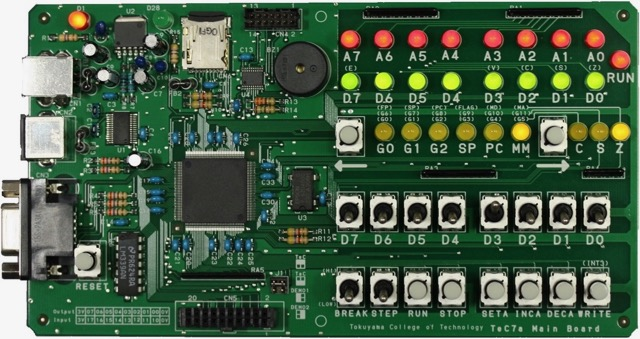
\includegraphics[scale=0.35]{Photo/TeC7.jpg}\\
(a) TeC7の写真
\end{center}
\end{minipage}
\begin{minipage}{0.38\columnwidth}
\begin{center}
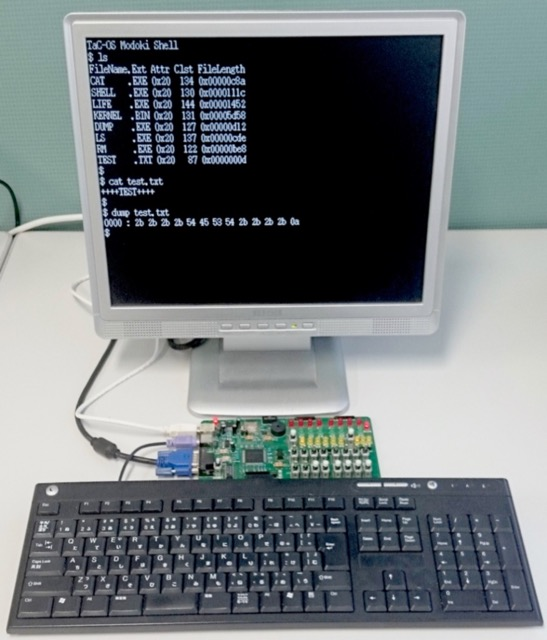
\includegraphics[scale=0.29]{Photo/TaC.jpg}\\
(b) TaCとしての使用例
\end{center}
\end{minipage}
\end{myfig}

TaC上では{\cmm}言語\footnote{
C言語に似た言語,
詳細は\url{https://github.com/tctsigemura/C--/blob/master/doc/cmm.pdf}を
参照のこと.}で記述されたTacOS\footnote{
詳細は\url{https://github.com/tctsigemura/TacOS}を参照のこと.} が動作する.
本書ではTacOSをオペレーティングシステムの実装例として参照する.

\subsection{ハードウェア構成}
\figref{tacBlock}にTaCのハードウェア構成を示す.
16ビットのシングルプロセッサ(CPUが一つ),
主記憶64KiBの非常に単純なシステムである.
単純なのでオペレーティングシステムの構築も容易である.
TaCに関する資料を付録\ref{appTac}にまとめる.

\myfigure{btp}{scale=0.48}{Fig/tacBlock-crop.pdf}
{TaCのハードウェア構成}{tacBlock}

\begin{itemize}
\item {\bf コンソールパネル} \\
\figref{tacPhoto}「(a) TeC7の写真」で,
TeC7本体右半分のランプやスイッチで構成される部分をコンソールパネルと呼ぶ.
コンソールパネルはCPUや主記憶と直接接続されており,
CPUを停止した状態で,
CPUや主記憶の内容を操作したり観察したりすることができる.
また,機械語命令を一命令毎に実行するステップ実行機能や,
ある番地の命令を実行した時点でプログラムを停止する
ブレーク機能ポイントが利用できる.
コンソールパネルの機能はハードウェアで実現されているので,
オペレーティングシステムの内部をステップ実行することも可能である.
TacOSの開発では,コンソールパネルがデバッグに活用された.

\item {\bf CPU} \\
\figref{tacRegPsw}に示すようなCPUレジスタとPSWを持つ16ビットCPUである.
PSWのフラグに実行モードを表すPビットを持ち,
カーネルモードとユーザモードを切り換えることができる.
機械語命令は,\figref{tacInsTbl}に示す46種類が準備されている.
機械語命令のアドレッシングモードは8種類ある.

\item {\bf メモリ} \\
メモリは\figref{tacMap}に示す構成である.
メモリ空間全体で64KiB,
自由に使用できるメモリが56KiB,
2KiBのVRAMと4KiBのIPL,32Bの割込みベクタからなる.
メモリは8ビット単位,または,16ビット単位で読み書きできる.
16ビット単位の場合は偶数アドレスを用いる.

\item {\bf タイマー} \\
$1$ミリ秒から$2^{16}-1$ミリ秒までの間隔で割込みを発生する
インターバルタイマーが二つ利用可能である.

\item {\bf ディスプレイアダプタ} \\
80文字×24行の文字をVGAディスプレイに表示する.
メモリ空間の{\tt E000h}から配置されるVRAMに書き込んだ
ASCIIコードと対応する文字をディスプレイに表示する.
{\tt E000h}番地がディスプレイの左上隅に対応する,
{\tt E001h}番地が一行目の2文字の位置,
{\tt E04Fh}番地が一行目の80文字の位置,
{\tt E050h}番地が二行目の1文字の位置に対応する.

\item {\bf SPIホストコントローラ} \\
スロットに挿入されたマイクロSDカードをSPIモードに切換え読み書きを行う.
SPIホストコントローラに初期化コマンドを発行すると,
マイクロSDカードをSPIモードに切換える.
ブロックアドレスとメモリアドレスを設定して読み出しコマンドを発行すると,
マイクロSDカードの指定したブロックから512バイトのデータを
CPUを介さずに(DMA:Direct Memory Accessを用いて)メモリに読み出す.
書込みコマンドを発行すると,
メモリから指定ブロックにデータを書き込む.

\item {\bf シリアル通信インタフェース} \\
調歩同期方式,9,600Baudの通信インタフェースである.
USBシリアル変換ICを通してPC等のシリアルターミナルと通信できる.
1バイト転送する毎に割込みを発生する.

\end{itemize}

\subsection{TacOS}
\myfigure{btp}{scale=0.66}{Fig/tacosOrganization-crop.pdf}
{TacOSの構成}{tacosOrganization}

\figref{tacosOrganization}にTaC用のOSであるTacOSの構造を示す.
マイクロカーネルがプロセス間通信(IPC)機能を提供し,
サーバプロセスがメモリ管理やファイルシステム機能を提供する.
\figref{microkernel}の一般的なマイクロカーネル方式と異なり,
サーバプロセスがカーネルモードで動作しハードウェアに直接アクセスする.
また,サーバプロセスはマイクロカーネルと同じアドレス空間で動作するので,
カーネル内ルーチンをCALL機械語命令で直接に呼び出すことができる.

割込みやSVC命令の実行が原因で,
ユーザプロセスはカーネルモードに切り換わり
マイクロカーネル内の割込みハンドラが呼び出される.
割り込みハンドラで割込み原因を判断し,
マイクロカーネル内のルーチンを呼び出したり,
サーバプロセスの機能をIPCを用いて呼び出したりする.

\section{もう一つの仮想マシン}

\ref{osRole}で述べたように,
オペレーティングシステムは抽象化され便利な拡張マシン(仮想マシン)を,
必要な数だけ提供する.
ここで述べた仮想マシンは,単一ユーザ・プロセスの実行環境のことである.
同じ「仮想マシン」と言う用語が,
オペレーティングシステムを実行することが可能な,
よりハードウェアを忠実に再現した仮想マシンを指す場合もある.
ここでは,
一台のコンピュータ上で複数のオペレーティングシステムを実行可能な,
もう一つの仮想マシンについて紹介する.

\subsection{Type 2 ハイパーバイザ}
例えば,
Macを使用している人がWindowsでしか動作しないアプリケーションを使用する
場合を想像してしてみる\footnote{
徳山高専情報電子工学科のパソコン室では,
WindowsやLinuxでしか動作しないXilinx ISE WebPACKをMacで使用している.}.
予めMacのハードディスクにmacOSとは別にWindowsもインストールしておき,
電源投入時にmacOSとWindowsを選んでブートする方法もあるが,
オペレーティングシステムを切換える度にコンピュータを再起動するのは不便である.
また,macOSのアプリケーションとWindowsのアプリケーションを同時に実行したい
場合もある.

そこで,\figref{type2Hypervisor}に示すような
「Type 2 ハイパーバイザ(Type 2 Hypervisor)」を用いた仮想化が用いられる.
ハイパーバイザは
{\bf ホスト・オペレーティングシステム}の一つのユーザプロセスとして実行され,
コンピュータ一台の機能をエミュレーションする.
ハイパーバイザがエミュレーションするコンピュータの中で,
{\bf ゲスト・オペレーティングシステム}が稼働する.
エミュレーションはソフトウェアだけで完全に行うのではなく\footnote{
完全にソフトウェアで行う場合もある.},
ハードウェアの支援を受けて行うので高速に行うことができる\cite{virtualization}.
Type 2 ハイパーバイザとして有名は製品は,
VMware Workstation,
VMware Fusion,
VirtualBox\footnote{
徳山高専情報電子工学科のパソコン室では
macOS上のVirtualBoxでWindowsを動作させている.
%このWindowsの中でXlinix ISE WebPACKが使用できる.
}等である.

\myfigure{btp}{scale=0.66}{Fig/type2Hypervisor-crop.pdf}
{Type 2 ハイパーバイザ}{type2Hypervisor}

\subsection{Type 1 ハイパーバイザ}
メインフレーム上で1960年代から使用されている方式である.
現在ではPCサーバの仮想化にも使用されている.
Type 1 ハイパーバイザはホスト・オペレーティングシステム無しに
ハードウェア上で直接実行される.
Type 1 ハイパーバイザとして有名な製品は,
IBM z/VM,
VMware vSphere,
Xen,
Hyper-V等である.

サーバ向けの製品が主流であり,
例えば VMware vSphere は
実行中のゲストを他の物理サーバに移動する等,
非常に高度な機能を持っており\cite{vsphere},
一台のサーバ上に効率よく多数の仮想マシンを動かすことができる.
徳山高専情報電子工学科のパソコン室でも,
2台のサーバ上に50台の仮想デスクトップマシンを動かしていたことがある.

\myfigure{btp}{scale=0.66}{Fig/type1Hypervisor-crop.pdf}
{Type 1 ハイパーバイザ}{type1Hypervisor}

\subsection{仮想アプライアンス}
ゲスト・オペレーティングシステムとアプリケーションまでインストールし,
すぐに使用できる状態で配布される仮想マシンである.
例えば,メールフィルタソフトをインストールした仮想マシンを
入手しハイパーバイザで実行するだけですぐにメールフィルタリングが開始できる.

同じ手法で,
すぐに使用できるパーソナルコンピュータ用の
デスクトップ・オペレーティングシステムが配布されている場合もある.
Linux の一種であるUbuntuの場合,
VirtulBoxですぐに実行できるディスクイメージがダウンロードできる\cite{ubuntu}.
仮想アプライアンスは,
ソフトウェアの新しい流通手法である.

\section{まとめ}
本書は{\bf SMP(対称型マルチプロセッシング:Symmetric Multiprocessing)}の
コンピュータを前提にしている.
CPUは{\bf PSW(Program Status Word)}と{\bf CPUレジスタ}を含んでいる.
最近のIntel社のCPUでは,従来のCPUを{\bf Core(コア)},
複数のコアを含んだLSIのことをCPUと呼ぶ.

オペレーティングシステムのカーネルは,
割込みハンドラ,ディスパッチャ,サービスモジュール,
デバイスドライバ等から構成される.
ユーザ・プロセスからカーネルへの切換え原因は{\bf 割込み}だけである.
ユーザ・プロセス毎に{\bf 仮想CPU},{\bf 仮想メモリ空間},管理情報等を
持っている.

カーネルの構成方式には,
{\bf 単層カーネル(モノリシック・カーネル)}方式と
{\bf マイクロカーネル(micro-kernel)}方式の二種類があった.
マイクロカーネル方式ではサービスモジュールをサーバ・プロセスとし,
{\bf IPC(プロセス間通信)}を用いてサービスを要求する.
サービスモジュール間の独立性が高くなり高信頼性のシステムを構成可能であるが,
IPCはオーバーヘッドが大きい.
信頼性と性能はトレードオフの関係にある.

{\bf TaC}は,本書でオペレーティングシステムの実装例として使用する
TacOSを稼働させるコンピュータである.
コンソールパネルを持ち,
TacOSのカーネル内までステップ実行によるトレースが可能である.
{\bf TacOS}はマイクロカーネル方式の簡単なオペレーティングシステムである.
本書では,しばしばTacOSのソースコードを実装例として参照する.




